
%(BEGIN_QUESTION)
% Copyright 2006, Tony R. Kuphaldt, released under the Creative Commons Attribution License (v 1.0)
% This means you may do almost anything with this work of mine, so long as you give me proper credit

Forklar hva denne elektriske magnetventilen vil få den pneumatisk aktuert reguleringsventilen til å gjøre når den spenningsløses. Hvilken type failsafe-modus gir denne magnetventilen reguleringsventilen som ventilen ellers ikke ville hatt på egen hånd?

$$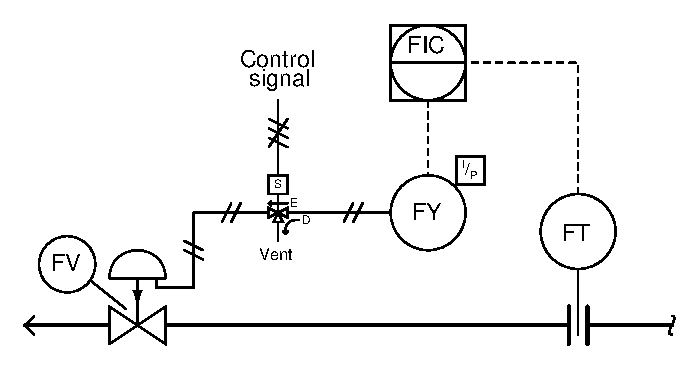
\includegraphics[width=15.5cm]{i00917x01.eps}$$

Ut fra hvordan væskestrømregulatorer normalt tunes: hvordan vil regulatoren (FIC) reagere i automatisk modus hvis magnetventilen ``tripper''?

\vskip 20pt \vbox{\hrule \hbox{\strut \vrule{} {\bf Forslag til sokratisk diskusjon} \vrule} \hrule}

\begin{itemize}
\item{} Hvilken prosesstype er væskestrøm: {\it selvregulerende}, {\it integrerende}, eller {\it runaway}?
\item{} Ideelt sett, hvordan bør en væskestrømregulator tunes?
\end{itemize}

\underbar{file i00917}
%(END_QUESTION)





%(BEGIN_ANSWER)


%(END_ANSWER)





%(BEGIN_NOTES)

Når magnetventilen er spenningsløs, vil den få reguleringsventilen til å ``låse'' i posisjon og ikke svare på utgangssignalet fra I/P-transduseren.

\vskip 10pt

Magnetventilen gir en ``fail in place''-modus for reguleringsventilen. Ventilen alene er en fail-close-konstruksjon (slik pilen på stammen viser).

\vskip 10pt

Hvis magnetventilen tripper og i praksis kobler reguleringsventilen fra regulatoren, vil regulatoren mest sannsynlig ``wind up'' eller ``wind down'' på grunn av aggressiv integralvirkning. Den eneste måten dette {\it ikke} skjer på er om flowen tilfeldigvis stabiliserer seg nøyaktig på settpunkt idet ventilen tripper, noe som er lite sannsynlig.

\vskip 20pt \vbox{\hrule \hbox{\strut \vrule{} {\bf Virtuell feilsøking} \vrule} \hrule}

Denne oppgaven egner seg godt som en ``virtuell feilsøkings''-øvelse. Når du presenterer diagrammet for studentene, forestiller du deg først en bestemt feil i systemet. Deretter presenterer du ett eller flere symptomer på denne feilen. Studentene foreslår ulike diagnostiske tester for å identifisere feilens art og plassering, som om de var teknikere som feilsøker problemet. Din jobb er å fortelle hva resultatet blir for hver foreslåtte test.

Under og etter øvelsen er det nyttig å stille oppfølgingsspørsmål som:

\begin{itemize}
\item{} Hva forteller resultatet av den siste diagnostiske testen om feilen?
\item{} Anta at resultatet av den siste diagnostiske testen hadde vært annerledes. Hva ville det da fortalt om feilen?
\item{} Er den siste diagnostiske testen den beste testen vi kunne gjort?
\item{} Hva ville vært ideell testrekkefølge for å diagnostisere problemet med færrest mulig trinn?
\end{itemize}

%INDEX% Final Control Elements, valve: fail-safe solenoids

%(END_NOTES)

